\documentclass[12pt,a4paper] {report}

% Packages
\usepackage{graphicx}
\usepackage{amsmath}
\usepackage{hyperref}
\usepackage{setspace}
\usepackage{listings}
\usepackage{xcolor}  % Include xcolor for text color

\lstset{
  literate={\_}{{\_}}{1},   % Replace _ with the literal \_
  basicstyle=\scriptsize\ttfamily,      % Optional: Set typewriter font for listings
  breaklines=true,            % Enable line breaking for long lines
  postbreak=\mbox{\textcolor{red}{$\hookrightarrow$}\space}, % Optional: indicate line break
  literate={|}{{\textbar}}1 {0}{{0}}1 {>}{{\textgreater}}1 {\_}{{\_}}1,
  escapechar=\%             % Optional: Set an escape character if needed
}
% Title and Author (adjust the spacing as needed)
\title{\LARGE \textbf{Quantum Networking: Explore QKD and quantum internet}}
\author{}
\date{\large On: \today}

% Begin Document
\begin{document}

% Title Page
\makeatletter
\begin{titlepage}
\centering
\vspace* {1cm}
{ 
\includegraphics[width=6cm]{ELMEPA.png}}\\[1cm]

{\LARGE \textbf{Quantum Networking: Explore QKD and quantum internet}}\\[1cm]
Project for\\[1cm]

	Advanced Networks Master's program course\\[0.5cm]



	\textbf{Written By:} {Nikolaos Mouzakitis MTP321}\\[1cm]
\date{\large Date Last Edited: \today}
{\@date\\}
\end{titlepage}
\makeatother
% Abstract


	\chapter* {Abstract}
	\addcontentsline{toc} {chapter} {Abstract}

		Quantum networking represents a transformative advancement in secure communication,
		with Quantum Key Distribution (QKD) and the quantum internet standing at its core.
		Unlike the widely available and adopted classical systems, QKD leverages certain mechanical principles
		from the field of quantum physics in order to theoretically guarantee unbreakable encryption schemes,
		addressing critical vulnerabilities in modern cryptographic methods.
		In the early days of its rise, quantum internet promises a global network enabling unprecedented levels of
		secure communication, distributed quantum computing, and advanced scientific applications.

% Table of Contents
\tableofcontents

        % Chapters
        \chapter{Introduction}

		Quantum networking stands as the next frontier in communication technology,
		which is expected to leverage principles of quantum mechanics for
		achieving unprecedented levels in security, as well as in computational capability.
		In contrast to ordinary classical networks, quantum networks rely on quantum states
		of the likes of superposition and entanglement to achieve operations impossible for
	        the classic networking schemes. These attributes become of vital importance in 
		application areas like secure communications, where quantum key distribution (QKD) 
		promises provable security against eavesdropping, and in distributed computing in cases 
		where quantum nodes could collaborate to solve problems beyond the reach of classical networks.
		In the modern world, where the requirement for global data security keeps following
		an increasing trend, quantum networking is considered as a robust solution
		for protecting sensitive informations.
		Moreover, it is possible that mixed architectures combining classical and quantum network elements
		could provide a feasible solution for the future communication systems. 
		To define the structure and complete functionality of the future quantum internet,
		a complete network stack is required to be created starting from the beginning utilizing 
		the features of quantum entanglement\cite{rfc}.

		Challenges arise although; despite the promising potential in quantum networking,
		it faces technical and theoretical obstacles that need to be surpassed
		in order to achieve and enable an entirely practical implementation and adoption.
		Because of the very nature of quantum mechanichs, quantum internet is opted to utilize concepts
		without classical counterparts with the likes of quantum entanglment,
		no-cloning theorem, quantum measurement and teleportation.
		
		In contrast to the classical and well known model of computation experienced so far,
		where we deeply rely on the fact that information can be read and copied, this concept that does not hold
		for quantum networking. 
		
		The scalability remains one of the main issues,
		because as current quantum networks are limited in the number of nodes and the
		distances they can span without degradation.
		This limitation comes from the fragile nature of the quantum states,
		which are very sensitive on environmental noise and decoherence especially over long distances.
		As a countermeassure, in order to avoid these limitations the development of reliable quantum repeaters
		and advanced error-correction schemes are required.	
		Additionally, the efficient generation, distribution and storage of entanglement 
		across a network has its difficulties and limitations that are required to be surpassed, 
		as maintaining a high fidelity value in entangled
		states is necessary for a complete and functioning network.
		In the end, another challenge lies in integration
	        quantum systems with the classic infrastructure,
	        which requires coordination between
	        two different operational paradigms.
	        Addressing these challenges is critical for the transission of 
		quantum networking from the experimental level to real-world applications.

		In this project the current state of quantum networking is explored alongside its potential applications. 
		The introduction provides a broad overview of the field, emphasizing its importance in secure communication and presents a brief
		description of the most common terminology of quantum networking.	
		In the related work section recent advancements in quantum networking are presented, with a focusing on technologies such as 
		quantum key distribution, entanglement distribution, and quantum repeaters. 
		In the combined methodology and results section, a simulation-based approach utilizing QuTiP 
		showcases examples to study the key elements of quantum networking, presenting the findings from the simulations.
		The discussion section interprets these findings in the context of existing literature, 
		identifying both strengths and limitations of current technologies. 
		In the end, the conclusion section summarizes the project's work.


		\section{A brief description of the most common terms in quantum networking}

		A \textbf{quantum network} consists of a set of quantum processors/devices connected to each other. \textbf{Qubits} can be particles such as photons
		or electrons, carrying certain properties derived from quantum mechanics called \textit{state}. A state's can express the spin of an electron or
		a photon's polarization. The particular state of a qubit is unknown prior to its measurement, since it is in a 
		superposition (\textit{as an analogy one can think the linear combination of two variables)} of states.
		After its measurement the qubit collapses in one state, which actually can not be determined
		before since it is related with the basis that is used in the measurement.
		
		\textbf{Quantum superposition} consists one of the ground principles in quantum mechanics. 
		It presents the property that quantum system has, of existing in multiple states at the same time, until it gets measured. 
		Superposition denotes that prior to measurement, the system does not exist in any state but in a combination of both states.
		States in quantum mechanics are denoted as $|\psi\rangle$ and represent a vector in a complex Hilbert space. 
		A system in superposition is described as a linear combination of basis states:
			\[
			|\psi\rangle = a_0 |0\rangle + a_1 |1\rangle,
			\]
		where:
		\begin{itemize}
			\item $|0\rangle$ and $|1\rangle$ are the basis states, and
			\item $a_0$ ,$a_1$ belong to complex numbers and satisfy the following equation:
			\[
			|a_0|^2 + |a_1|^2 = 1.
			\]
		\end{itemize}

		Coefficient $|a_0|^2$ represent the probability of measuring the system state as $|0\rangle$ and $|a_1|^2$ the probability to measure it
		as $|1\rangle$. After describing its properties, we can understand why superposition constitutes a 
		basic difference in between quantum and classical mechanics. 

		\textbf{Quantum entanglement} is the situation where two qubits become correlated
		(called \textit{entanglement pair}) in a way that
		any modification on the state of the first at once affect the state, and is reflected on the second qubit, 
		without any consideration of their actual distance. Because of the no-cloning theorem, there it is not even
		possible for a third qubit to be entangled with either of those qubits. Close tied to entanglement, the concept
		of \textbf{quantum teleportation} is a process, in which state information of a quantum particle can be transferred
		from one location into another without that particle beeing trasported.
		This incident is feasible due to the entanglement.
		
		Another important property is the \textbf{fidelity} of a quantum state.
		Fidelity is a metric  \( \textit{f} \in [0,1] \), denoting the quality of a quantum state.
		The higher the value is, the closer the quantum state is to what it was created to be.
		Fidelity represents this probability, allowing the evaluation of how much environmental noise
		and losses have impacted the quantum state.

		The \textbf{no-cloning theorem} is a fundamental principle in quantum mechanics 
		which states that it is impossible to create an exact copy of an unknown quantum state. 
		This theorem has important consequences in quantum information theory and especially in
		quantum cryptography and networking. The theorem therefore guarantees the secure quantum communication 
		in protocols such as Quantum Key Distribution (QKD) because it is impossible for any eavesdropper who copies
		quantum states in order to intercept informations to operate unnoticed.

		\section{QKD}
		Quantum Key Distribution is an approach of sharing and establishing a secret cryptographic key 
		among two communicating entities\cite{powergrid}.
		In order to achieve the desired outcome it utilizes both a quantum channel and a classical channel 
		of communication. The quantum one is used to transmit qubits among the entities while the classical 
		one operates for establishing the final key and for encrypted data exchanges following the classical 
		paradigm. QKD is only used for the generation of the initial key.

		\section{Quantum Repeaters}
		
		Quantum repeaters are devices which are designed to extend the range of quantum communication networks. They 
		are required to enable QKD in long distances and for supporting the construction of a future quantum internet.
		In the classical way of communication, the repeaters are used in order to amplify signals 
		for avoiding signal loss, but due to the no-cloning theorem which prohibits duplication of quantum states,
		this is not applicable on quantum communication. So a quantum repeater in constrast, utilizes entanglement distribution 
		and error correction schemes to achieve the establishment of a quantum connection over long distance.
		The main issues that quantum repeaters address are the following:

		\textbf{a)} Photon Loss (Attenuation):
		In fact, quantum repeaters can help to tackle the loss in fiber-based quantum communication,
		where the photons who carry quantum information experience loss inside the medium by propagation. 
		This limits the range of QKD to about tens of kilometers \cite{repeater1}. 
		By using them, and creating shorter segments with the interference of quantum repeaters in the medium,
		entanglement pairs can be created and saved for each segment, 
		and by using the technique of entanglement swapping, information can 'pass' through and realize a long distance connection.

		\textbf{b)} Decoherence:
		Quantum states are very sensitive and affected by environmental noise, forcing the states to lose coherence (\textit{preservation of quantum
		state over time and long distances}).
		Quantum repeaters use quantum memories\cite{memories} as intermediate nodes to store entangled states 
		temporarily, allowing processes such as error correction or entanglement purification to maintain 
		the quality of the entanglement.
		
		\textbf{c)} Scalability of Quantum Networks:
		Without using repeaters, quantum networks have to be limited small local areas due to the
		constraints of photon transmission.
		Quantum repeaters can enable a scalable construction 
		of larger quantum networks by bridging long distances using segmented 
		paths with entangled pairs connecting multiple nodes.
		
		\textbf{d)} Error Accumulation:
		In quantum communications, errors tend to accumulate over long distances
		and the classical error correction schemes are not applicable for the quantum states.
		Quantum repeaters integrate error correction protocols like entanglement purification
		in order to tackle this issue.

		\section{Bell state measurement}

		A Bell State Measurement (BSM) is a quantum operation designed to determine
		the entangled state of two qubits. The set of Bell states consists of four 
		maximally entangled quantum states representing the strongest correlations
		among two qubits. These states are:

			\begin{align*}
			    \Phi^+ &= \frac{1}{\sqrt{2}} (|00\rangle + |11\rangle), \\
			    \Phi^- &= \frac{1}{\sqrt{2}} (|00\rangle - |11\rangle), \\
			    \Psi^+ &= \frac{1}{\sqrt{2}} (|01\rangle + |10\rangle), \\
			    \Psi^- &= \frac{1}{\sqrt{2}} (|01\rangle - |10\rangle).
			\end{align*}

		In a BSM operation, the states of two qubits are projected onto one of these four Bell states. 
		As an outcome, information occurs about how the two qubits are related, but not information
		about their respective individual states. Their ability to manage and process entanglement
		in quantum networks establishes BSMs to be a critical element on the future quantum architectures.
		
		\section{Network Devices}
		e-qnet continue

\chapter{Related Work}
		In recent years, quantum networking has gained
		significant attention due to its potential to ignite a revolution in
		secure communications and distributed computing.
		Khristo et al. \cite{Khristo2020} have provided an overview of the field's
		current status but also of the desired future directions.
		In their work the key advancements and challenges in the
		development of quantum networks have been discussed while in addition
		explored the integration of the quantum key distribution (QKD)
		and presented a broader vision for the quantum internet.
		
		Kozlowski et al. \cite{rfc} focus on presenting the architectural foundations required in order to
		realize the quantum internet, strongly proposing the incorporation of quantum entanglement and Bell pairs for quantum networks. 
		The different aspects among quantum and classical networks are discussed, while authors point out the use of hybrid
		classical-quantum architectures. Van Meter et al. \cite{quantum-arch} proposed a complete architecture 
		for a scalable unified quantum communications. They utilize a two-pass connection setup and recursive protocol
		to allow scalability and extensibility for future internetworking
		of many quantum devices. Authors also presented protocols-algorithms for connection establishments, desicion making, routing and 
		allocation of resources inside the quantum network and its consisting layers.
		Quantum internet concept is also been explored by Cacciapuoti et al. \cite{net-chall-dqc}.
		In their work the key differences among quantum and classical
		networks ar underlined, and point out quantum teleportation as the most fundamental method of transporting 
		informations in a quantum system. Authors proposed a framework for tackling the challenges of a quantum
		network creation as well as emphasizing on the need to address problems like decoherence for enchancing the
		reliability these networks. The key role of quantum teleportation is also discussed in \cite{entagl-classic},
		where authors recommend a redesignation of the classic communication paradigm in order to conform with the quantum teleportation needs.
		They describe the generation and distribution of entanglement by using photons for transmissions, and propose certain schemes for extending
		the range of communications such as the entanglement swapping.

		%Repeaters
		In contrast to traditional quantum repeaters who require the use of entaglement swapping and quantum memory, all-photonic quantum repeaters
		are based on light particles(photons) for the transfer of quantum information.
		Authors in \cite{repeater1} propose an all photonic quantum repeater 
		based on RGS (repeater graph states) achieving a higher repetition rate compared to traditional quantum repeaters, and does not require 
		the use of quantum memories. Their proposed scheme offers a fast Bell pair generation ration with only
		limitation the time required for the creation of the repeater graph state. 
		As per quantum memories, in their work Bhaskar et al. \cite{memories}, demonstrated a quantum memory node, which
		was integrated into a nanophotonic resonator. Their memory node, was able to perform asynchronous Bell-state measurements
		and proved that their setup is outperforming direct methods of transmission.
		

		In another step towards the realization of a complete quantum network architecture,
		researchers have implemented complete protocol stacks for quantum networks.
		Pompili et al. \cite{pompilli} have experimented with entanglement delivery across 
		a network's protocol stack and proposed a division of it, in order to provide 
		independency between the physical implementation and the uppermost layers. 
		In this way the protocol stack is splitted into Physical and Platform-Independent
		(Hardware abstraction layer, Link layer, Network layer, Application layer).

		
		%other appliances-powergrid to cite.
		There ...  \cite{powergrid}







	\chapter{Methodology and Results}
		
		For the purposes of this project, a
		simulation approach using software tools
		have been employed in order to enable the
		demonstration of selected concepts in quantum networking.
		QuTiP(Quantum Toolbox in Python)\cite{qutip}, an open source framework
		written in Python, has been used for the simulations.

		\section{BB84 Quantum Key Distribution Protocol}

		BB84 protocol is a foundational work in the field
		of quantum key distribution (QKD) protocols,
		been proposed back in 1984 \cite{bb84}.
		It realizes a secure communication of a secret cryptographic key
		alongside two entities, over a potenitally insecure medium/channel
		by using principles of quantum mechanics.
		
		In this simulation (code is in Listing 1 of Appendix A),
		two entities entitled Alice and Bob, execute the QDK using the BB84 protocol
		in order to share a secret key over a potentially non-secure medium. Initially Alice creates
		a number of qubits (100 in this example) randomly in one of the two possible bases (either 'x' or 'z') and sends them 
		to Bob. Bob on his side, randomly selects a base per qubit and measures it. In the next step, 
		they are comparing their used bases over a classical communication channel and 
		they discard all the bits generated as an outcome from the measured qubits whose bases were not matching.
		The remaining bits which obtained from matching bases among the two entities are kept and create the shared secret key.
		It is important to note, that the qubits measurements from the mismatched bases are 
		discarded, since the outcome of the measurement on a mismatched base is probabilistic,
		and this does not ensure an identical secret key for both parties.
		\begin{figure}[h!]
			\centering
			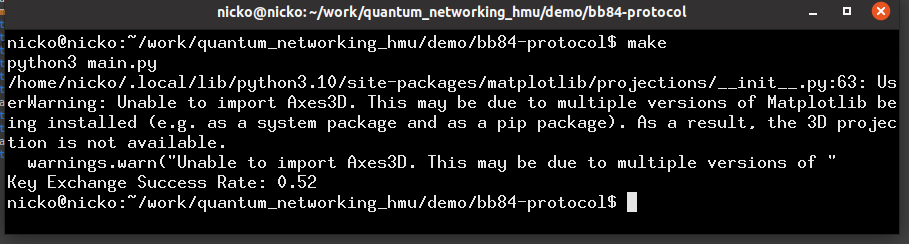
\includegraphics[width=0.8\textwidth]{bb84/success_rate_terminal.png}
			\caption{Execution of code of Listing 1 of Appendix A.}
			\label{fig:}
		\end{figure}		

		\begin{figure}[h!]
			\centering
			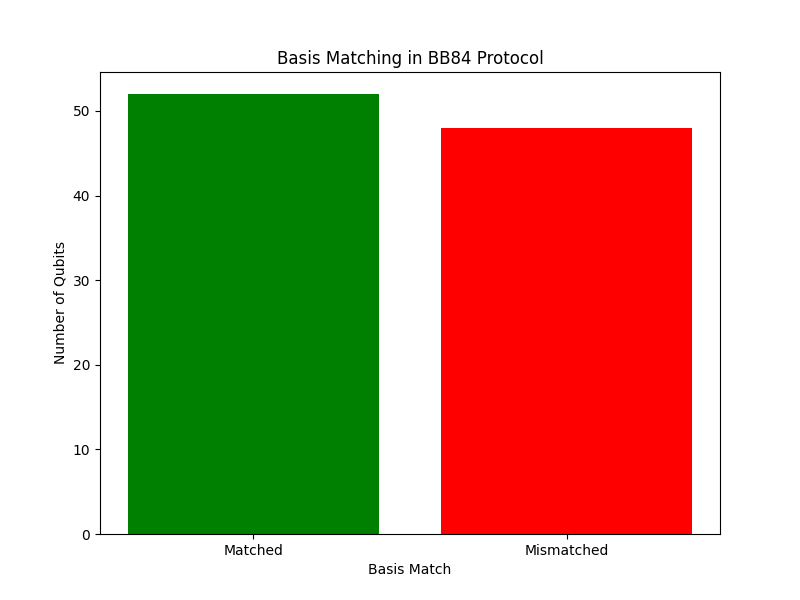
\includegraphics[width=0.6\textwidth]{bb84/basis_matching.png}
			\caption{Bases matched on the example where 100 qubits used.}
			\label{fig:}
		\end{figure}		


		\begin{figure}[h!]
			\centering
			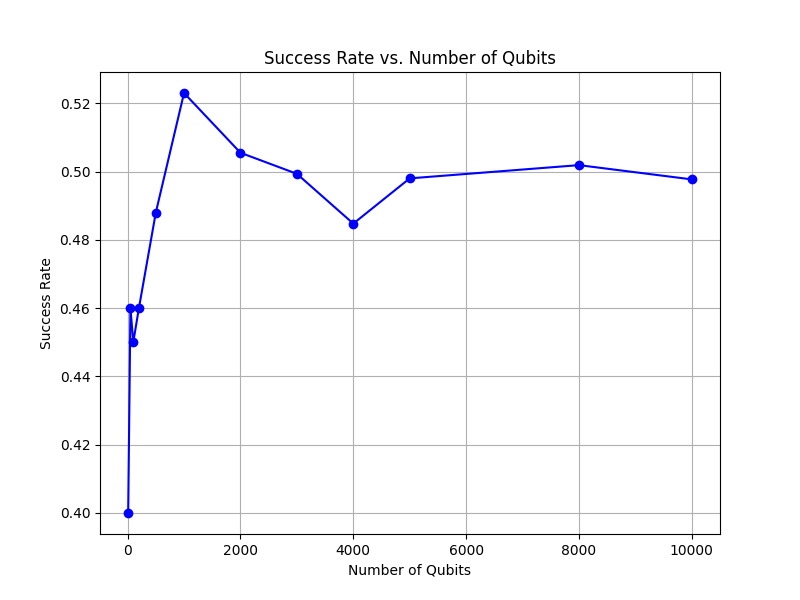
\includegraphics[width=0.6\textwidth]{bb84/success_rate_vs_num_qubits.png}
			\caption{Success rate vs number of qubits used.}
			\label{fig:}
		\end{figure}		

		As we can observe in Figure 3.3, the relation of success rate is plotted against the utilized 
		number of qubits in the protocol. The simulation was run for up to 10000 qubits. 
		Success rate is converging to value 0.5, as the probability 
		of Alice and Bob choosing the same base ('x' or 'z') is 50\%.

		\section{Fidelity against Noise Level}	
		
		In this simulation (code is in Listing 2 of Appendix A), a model of a quantum repeater network with
		entanglement swapping is created in order to observe how the fidelity of the final entangled state is
		affected by depolarizing noise \cite{depolarization}. Depolarizing noise is a quantum noise which models the
		coherence loss in quantum system's states because of imperfections in quantum operations.
		
		The depolarizing noise on a quantum state can be expressed as \cite{depolar2}:
			\[
			\rho \to (1-p)\rho + \frac{p}{d}I
			\]

		where:

		\begin{itemize}
			    \item \( \rho \): density matrix of quantum state before the noise is applied.
			    \item \( p \): depolarizing probability,  value \(\in [0, 1]\).
			    \item \( d \): Hilbert's space dimension. For a single qubit, \( d = 2 \).
			    \item \( I \): identity matrix \( d \times d \).
		\end{itemize}

		This form to model the noise is used in the presented simulation code.
	
		\begin{figure}[h!]
			\centering
			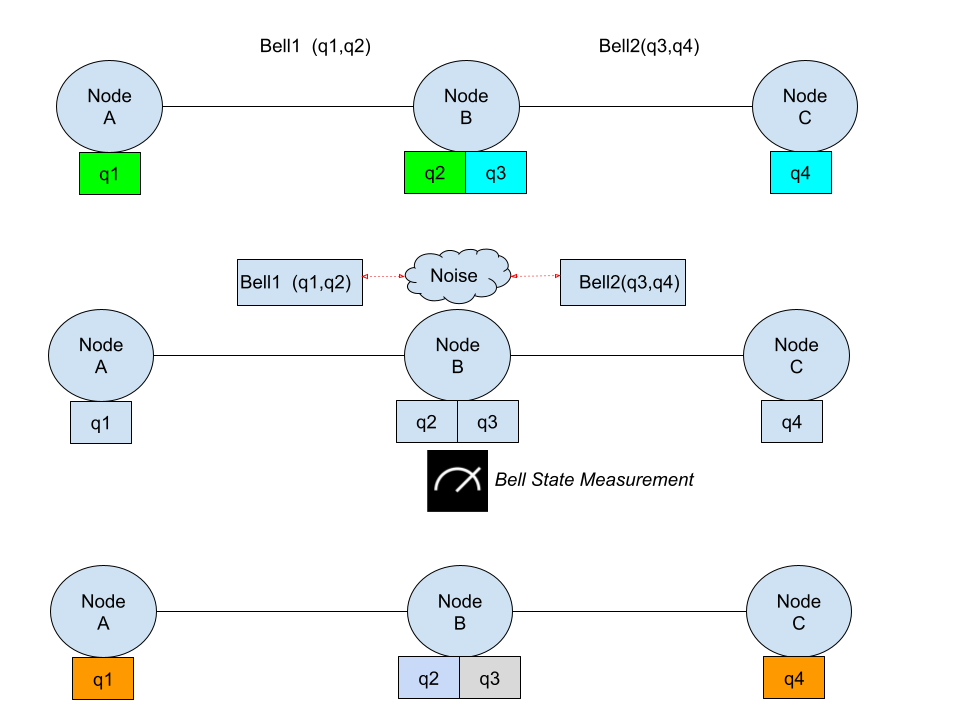
\includegraphics[width=0.7\textwidth]{repeater/entanglement_swap.png}
			\caption{Set up for the entanglement swapping}
			\label{fig:}
		\end{figure}		

		In the set up of Figure 3.4 we can inspect that qubits q1 (node A) and q2 (node B) are
		entangled in Bell1(Bell state 1) and q4 (node C) and q3 (node B) are entangled in Bell2(Bell state 2).
		Node A and Node C, could create these entangled pairs and sent 1 qubit each into the intermediate
		Node B. The BSM(measurement) occurs in Node B, and as a consequence the initial entanglement between
		q3 and q4 qubits is destructed \cite{rfc}. Nevertheless the state of q2 is "recreated"/reappears in the possition
		of qubit q4, which makes an new entanglement pair consisting of qubits (q1,q4).

		Depending on the application requirements, the results of the BSM might be communicated to the Node C, in order
		to apply a correction operation on q4 depending on which Bell state was received. More specifically, the measurement
		collapses the quantum states of q2 and q3, but it also results in a change in the state of q1 and q4.
		Qubits q1 (Node A) and q4 (Node C) become entangled as a result of the BSM, but they are not measured themselves.
		This is known as the process of entanglement swapping. Now (q1,q4) share an entangled state, even though they 
		were not directly entangled initially.

		Fidelity calculates how close the state is to the desired state. 
		As the noise in the system increases, the fidelity of the final state decreases,
		indicating the decrease in quantum entanglement quality.

		\begin{figure}[h!]
			\centering
			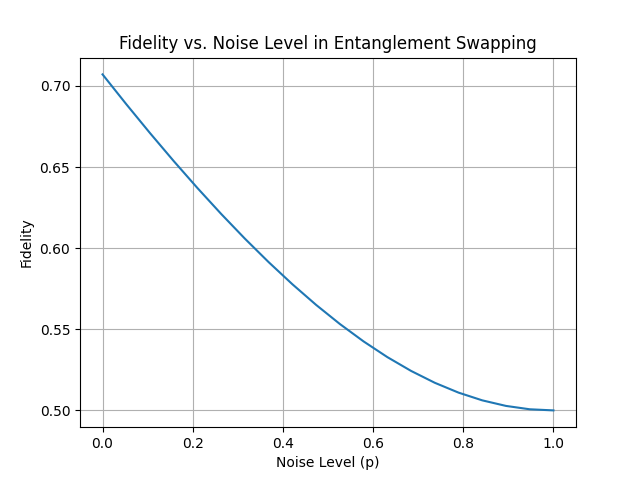
\includegraphics[width=0.6\textwidth]{repeater/fid_vs_noise.png}
			\caption{Fidelity vs Noise Level.}
			\label{fig:}
		\end{figure}		

		A value of 1 indicates the maximum perfect fidelity where there is no loss of entanglement, 
		while lower values indicate a degradation due to noise.
		In practice a fidelity value less than 0.5 indicates that the state is unsuitable for further quantum processing.
		In Figure 3.5 we can inspect that as the noise level increases, the fidelity decreases,
		an expected behavior since noise disrupts the quantum states,
		making the final entangled state less similar to the ideal state.




	\chapter{Discussion}

	\chapter{Conclusion}



\bibliographystyle{plain}
\bibliography{references}
\newpage
\appendix

\section*{Appendix A: Simulation Code }

%\begin{lstlisting}[language=Python, caption=BB84 for QKD, label=code:QKD, escapeinside=||]
\begin{lstlisting}[language=Python, caption=BB84 for QKD, label=code:QKD]
from qutip import basis, ket2dm
import numpy as np
zero = basis(2, 0)  ''' |0> '''
one = basis(2, 1)   ''' |1> ''' 
plus = (zero + one).unit()  ''' |+> '''
minus = (zero - one).unit() ''' |-> ''' 
''' Alice's qubits'''
def generate_bb84_states(num_qubits):
    states = []
    bases = []
    for _ in range(num_qubits):
        basis_choice = np.random.choice(['z', 'x'])
        bit = np.random.choice([0, 1])
        if basis_choice == 'z':
            states.append(zero if bit == 0 else one)
        else:
            states.append(plus if bit == 0 else minus)
        bases.append(basis_choice)
    return states, bases
'''Measurement'''
def measure_state(state, basis):
    if basis == 'z':
        projection = [zero, one]
    else:  ''' 'x' '''
        projection = [plus, minus]
    probabilities = [abs(proj.overlap(state))**2 for proj in projection]
    return np.random.choice([0, 1], p=probabilities)
'''Simulation'''
num_qubits = 100
alice_states, alice_bases = generate_bb84_states(num_qubits)
bob_bases = np.random.choice(['z', 'x'], num_qubits)
''' Measure and compare '''
bob_results = [measure_state(state, bob_bases[i]) for i, state in enumerate(alice_states)]
matching_bases = [alice_bases[i] == bob_bases[i] for i in range(num_qubits)]
shared_key = [bob_results[i] for i in range(num_qubits) if matching_bases[i]]
''' Calculate success rate'''
success_rate = len(shared_key) / num_qubits
print(f"Key Exchange Success Rate: {success\_rate:.2f}")
import matplotlib.pyplot as plt
''' Visualization 1: Basis Matching (Bar Chart)'''
matched = sum(matching_bases)
mismatched = num_qubits - matched
plt.figure(figsize=(8, 6))
plt.bar(['Matched', 'Mismatched'], [matched, mismatched], color=['green', 'red'])
plt.title('Basis Matching in BB84 Protocol')
plt.xlabel('Basis Match')
plt.ylabel('Number of Qubits')
plt.savefig('Basis Matching in BB84 Protocol.png')
''' Visualization 2: Success Rate vs. Number of Qubits (Line Chart) '''
num_qubits_list = [10, 50, 100, 200, 500, 1000, 2000, 3000, 4000, 5000, 8000, 10000]
success_rates = []
for nq in num_qubits_list:
    alice_states, alice_bases = generate_bb84_states(nq)
    bob_bases = np.random.choice(['z', 'x'], nq)
    bob_results = [measure_state(state, bob_bases[i]) for i, state in enumerate(alice_states)]
    matching_bases = [alice_bases[i] == bob_bases[i] for i in range(nq)]
    shared_key = [bob_results[i] for i in range(nq) if matching_bases[i]]
    success_rate = len(shared_key) / nq
    success_rates.append(success_rate)
plt.figure(figsize=(8, 6))
plt.plot(num_qubits_list, success_rates, marker='o', color='b')
plt.title('Success Rate vs. Number of Qubits')
plt.xlabel('Number of Qubits')
plt.ylabel('Success Rate')
plt.grid(True)
plt.savefig("Success Rate vs Number of Qubits.png")

\end{lstlisting}


\begin{lstlisting}[language=Python, caption=Entanglement swapping(fidelity vs polarizing noise), label=code:QKD]

from qutip import *
import numpy as np
import matplotlib.pyplot as plt

''' Define Bell state '''
def create_bell_state():
    zero = basis(2, 0)  
    one = basis(2, 1)   
    bell_state = (tensor(zero, zero) + tensor(one, one)).unit()  
    bell_dm = ket2dm(bell_state)  ''' Convert to density matrix, shape: (4, 4)'''
    return bell_dm

''' Apply noise to a quantum state (Depolarizing channel)'''
def apply_depolarizing_noise(state, p):
    dim = np.prod(state.dims[0])  ''' Total dimension of the system'''
    identity = qeye(dim)  ''' Identity operator, shape: (dim, dim)'''
    identity.dims = state.dims
    n1=(1-p)*state
    n2 = (p/dim)*identity
    noisy_state = (1 - p) * state + (p / dim) * identity
    return noisy_state

''' Entanglement swapping '''
def entanglement_swapping(bell1, bell2):
    """
    Perform entanglement swapping between two Bell states:
    bell1: A-B (shape: (4, 4)), bell2: B-C (shape: (4, 4))
    Returns:
    - swapped_state: final entangled state between A and C (shape: (4, 4))
    """
    # Bell measurement on qubits 2 and 3 (middle qubits)
    bell_meas = (tensor(basis(2, 0), basis(2, 0)).proj() + 
                 tensor(basis(2, 1), basis(2, 1)).proj())  # Bell basis, shape: (4, 4)
    projection = tensor(qeye(2), bell_meas, qeye(2))  # Operate on qubits 2 and 3, shape: (16, 16)
    
    # Combine the two input states into a joint density matrix
    joint_state = tensor(bell1, bell2)  # Combined state, shape: (16, 16)
    
    # Apply projection for entanglement swapping
    swapped_state = (projection * joint_state * projection.dag()).unit()  # Shape: (16, 16)
    
    # Partial trace over qubits 2 and 3 to get A-C state
    final_state = swapped_state.ptrace([0, 3])  # Shape: (4, 4)
    return final_state

# Network Simulation
def simulate_network():
    """
    Simulates a basic quantum repeater network with entanglement swapping.
    Returns:
    - fidelity_value: fidelity of the final entangled state with an ideal Bell state
    """
    noise_levels = np.linspace(0, 1, 20)  # Noise levels from 0 to 1
    fidelities = []


    ''' Step 1: Create initial entanglement between nodes'''
    bell1 = create_bell_state()  # Between nodes A and B
    print(bell1)

    bell2 = create_bell_state()  # Between nodes B and C
    print(bell2)
    
    ''' Step 2: Calculate fidelity for different noise levels '''
    for p in noise_levels:
        bell1_noisy = apply_depolarizing_noise(bell1, p)
        bell2_noisy = apply_depolarizing_noise(bell2, p)
        final_state = entanglement_swapping(bell1_noisy, bell2_noisy)
        ideal_bell = create_bell_state()
        print(ideal_bell)
        fidelity_value = fidelity(final_state, ideal_bell)
        fidelities.append(fidelity_value)
    
    ''' Step 3: Plot fidelity vs noise level'''
    plt.plot(noise_levels, fidelities)
    plt.xlabel("Noise Level (p)")
    plt.ylabel("Fidelity")
    plt.title("Fidelity vs. Noise Level in Entanglement Swapping")
    plt.grid(True)
    plt.savefig("Fidelity vs Noise Level in Entanglement Swapping.png")   

# Main Execution
if __name__ == "__main__":
    simulate_network()


\end{lstlisting}

\end{document}
